\chapter{Technical Background}

\section{ROS}

The Robot Operating System (ROS) is a flexible framework for writing robot software. It is a collection of tools, libraries, and conventions that aim to simplify the task of creating complex
and robust robot behavior across a wide variety of robotic platforms. 

ROS is an open-source, meta-operating system for your robot. It provides the services you would expect from an operating system, including hardware abstraction, low-level device control,
implementation of commonly-used functionality, message-passing between processes, and package management. It also provides tools and libraries for obtaining, building, writing, and running code across multiple computers.

The ROS runtime "graph" is a peer-to-peer network of processes (potentially distributed across
machines) that are loosely coupled using the ROS communication infrastructure. 
ROS implements several different styles of communication, including synchronous RPC-style communication over services, asynchronous streaming of data over topics, and storage of data
on a Parameter Server.

ROS is a distributed framework that enables executable to be individually catered and tailored
based on the needs of the developer and the design of the application. ROS also supports docker
platform for the ease of virtualization and deliver software in terms of Containers[2].

\begin{figure}[h]
	\begin{center}
		
\includegraphics[height=2.5cm]{images/ros_logo.png}
		\caption{ROS logo}
	\end{center}
\end{figure}


\section{Rosbag}

This is a set of toll which is used to playing and recording of the ROS topics. It is basically used for high performance and avoids de-serialization and re-serialization of the messages. Bags are a format for saving and playing back ROS message data. Bags are an important mechanism for storing data, such as sensor data, that can be difficult to collect but is necessary for developing and testing algorithms[3]. 

\section{Rosbridge}


Rosbridge makes ROS topics and services available over either pure TCP sockets or web-sockets as JSON messages. Rosbridge provides a JSON API to ROS functionality for non-ROS programs. There are a variety of front ends that interface with rosbridge, including a WebSocket server for web browsers to interact with. Rosbridge\_suite is a meta-package containing rosbridge, various front end packages for rosbridge like a WebSocket package, and helper packages[4].

\section{Websockets}

WebSocket is a computer communications protocol, providing full-duplex communication channels over a single TCP connection. The WebSocket protocol was standardized by the IETF as RFC 6455 in 2011, and the WebSocket API in Web IDL is being standardized by the W3C.


Unlike HTTP, WebSocket provides full-duplex communication.[5] Additionally, WebSocket enables streams of messages on top of TCP.


\section{REST-API}

A REST API (also known as RESTful API) is an application programming interface (API or web API) that conforms to the constraints of REST architectural style and allows for interaction with RESTful web services. REST stands for representational state transfer[5].

An API is a set of definitions and protocols for building and integrating application software. It’s sometimes referred to as a contract between an information provider and an information user—establishing the content required from the consumer which is referred as call and the content required by the producer as the response.
\pagebreak
\section{REST-API v/s Websockets}
In this section there is comparison between the REST-API and WebSockets
\begin{table}[!htbp]
\centering
\resizebox{\columnwidth}{2.5cm}{\begin{tabular}{|c|c|c|}
	\hline
	\textbf{The basis of Comparison}& \textbf{WebSocket}  & \textbf{REST-API}  \\
	\hline
	\textbf{HTTP}&The use of HTTP occurs in the initial connection.  & HTTP is a common protocol in RESTful web services. \\
	\hline
	\textbf{Communication}& Bi-directional  & Uni-directional \\
	\hline
	\textbf{Nature}& Socket-based & Resources based concept, rather than commands \\
	\hline
	\textbf{Scenario}& Real time and continuous communication  & Based on the service request \\
	\hline
	\textbf{Dependency}& IP address and port number & Based on HTTP protocol \\
	\hline
	\textbf{Cost}& Cost of communication is lower & The cost of communication is slightly higher that WebSockets  \\
	\hline
	\textbf{Performance}& Better with high loads & Great for occasional communication \\
	\hline
	\textbf{State}& Websocket is a stateful protocol & REST is based on HTTP, which is a stateless protocol. \\
	\hline
\end{tabular}}
\caption{Comparison of WebSocket and REST-API}
\end{table}

\section{RViz}

RVIZ is a ROS graphical interface that allows you to visualize a lot of information, using plugins for
many kinds of available topics. It is a powerful robot visualization tool. It provides a convenient GUI to
visualize sensor data, robot models, environment maps, which is useful for developing and debugging
your robot controllers. It provides a view of your robot model, capture sensor information from robot
sensors, and replay captured data. It can display data from camera, lasers, from 3D and 2D devices
including pictures and point clouds.

It is designed to visualize data from the ROS framework. It also runs as a ROS node that can subscribe
to topics and display the contents of these messages. This is mainly used to display sensor data, like
point cloud data from a LiDAR or infrared distance measurements that are published to this topic by the
sensor.

It was used to visualize published information from the robot and also used in a later stage to issue
commands to the robot for navigation purposes. The software was chosen because of its tight
integration with the ROS framework. Rviz makes use of a file format called Universal Robotic
Description Format (URDF). A URDF file describing the Tiago was used to describe the robot and its
capabilities to Rviz. URDF files are written in XML by using the macro language xacro. This made the
URDF files easier to maintain and to read.

ROS makes use of topics to send messages from a publisher to a subscriber. Gazebo published
simulation messages which were computed within the ROS framework and then published to Rviz for
visualization. 


\section{Docker}

Docker is a open platform for developing, shipping and running application. Docker helps to run the developed application to run independent of the infrastructure used to develop. All the application will run on the docker cloud platform. Hence it will be independent of the underlying OS.

\subsection{Docker architecture}
Docker uses a client-server architecture[8]. The Docker client talks to the Docker daemon, which does the heavy lifting of building, running, and distributing your Docker containers. The Docker client and daemon can run on the same system, or you can connect a Docker client to a remote Docker daemon. The Docker client and daemon communicate using a REST API, over UNIX sockets or a network interface. Another Docker client is Docker Compose, that lets you work with applications consisting of a set of containers.

\begin{figure}[h]
	\begin{center}
		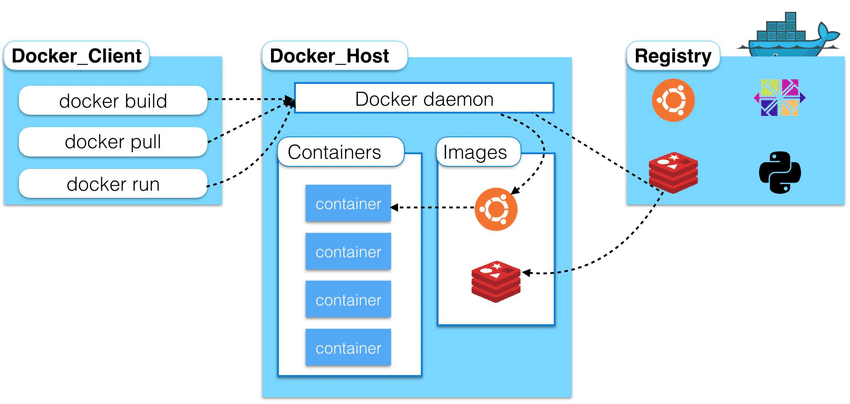
\includegraphics[height=10 cm,width=\linewidth]{images/docker_architecture.png}
		\caption{Docker Architecture}
	\end{center}
\end{figure}

\subsection{Docker objects}

When using Docker, we are creating and using images, containers, networks, volumes, plugins, and other objects. This section is a brief overview of some of those objects.


\onecolumn
\textbf{Images}

An image is a read-only template with instructions for creating a Docker container. Often, an image is based on another image, with some additional customization. For example, building an image which is based on the ubuntu image, but installs the Apache web server and our application, as well as the configuration details needed to make our application run.

We can also create our own images or we might only use those created by others and published in a registry. To build our own image, we create a Dockerfile with a simple syntax for defining the steps needed to create the image and run it. Each instruction in a Dockerfile creates a layer in the image. When we change the Dockerfile and rebuild the image, only those layers which have changed are rebuilt. This is part of what makes images so lightweight, small, and fast, when compared to other virtualization technologies.


\textbf{Containers}

A container is a runnable instance of an image. We can create, start, stop, move, or delete a container using the Docker API or CLI. We can connect a container to one or more networks, attach storage to it, or even create a new image based on its current state.

By default, a container is relatively well isolated from other containers and its host machine. You can control how isolated a container’s network, storage, or other underlying subsystems are from other containers or from the host machine.

A container is defined by its image as well as any configuration options you provide to it when you create or start it. When a container is removed, any changes to its state that are not stored in persistent storage disappear.

\section{VDA5050}

VDA 5050 is a standardized interface for AGV communication. Specifically, this standard concerns the communication between AGVs (often called Fahrerloser Transportsysteme/Transportfahrzeuge (FTS) in Germany) and a master control (in other words, a fleet management software program)[9].

In today's industries many AGV's of different manufacturers will be working together. Typically, these AGVs only work with their manufacturer’s own specific fleet management software. 

So some of the challenges arises in the industries such as

\begin{enumerate}
	\item Complex commissioning – a separate installation is needed for each brand of AGV
	\item Interoperability issues – it becomes difficult to manage AGVs if they need to cross paths or share an elevator say
	\item Lost space – separate AGV brands might need to use completely separate paths 
\end{enumerate}

Therefore VDA 5050 intends to provide a more generic version of this functionality, which would enable every compliant AGV to work together.

\begin{figure}[h]
	\begin{center}
		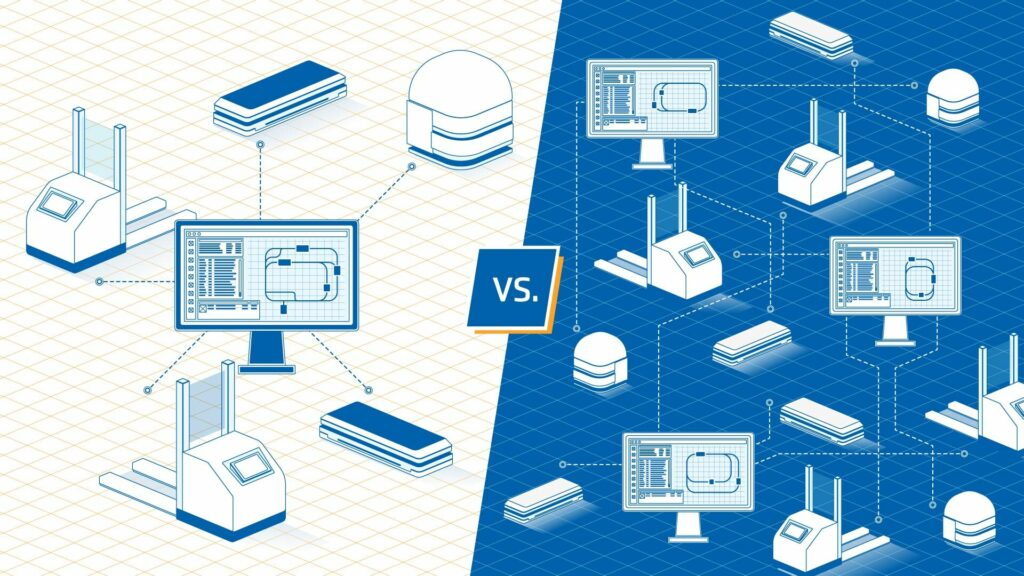
\includegraphics[height=10 cm,width=\linewidth]{images/vda.jpg}
		\caption{Main goal of VDA 5050 interface to bring most of the AMR in single Fleet}
	\end{center}
\end{figure}
\pagebreak
\section{CI/CD}

CI/CD is a method to frequently deliver apps to customers by introducing automation into the stages of app development. The main concepts attributed to CI/CD are continuous integration, continuous delivery, and continuous deployment. CI/CD is a solution to the problems integrating new code can cause for development and operations teams[10].

Specifically, CI/CD introduces ongoing automation and continuous monitoring throughout the lifecycle of apps, from integration and testing phases to delivery and deployment. Taken together, these connected practices are often referred to as a "\textbf{CI/CD pipeline}" and are supported by development and operations teams working together in an agile way with either a DevOps or site reliability engineering (SRE) approach.
\section{Webviz}

Webviz is a tool which is used to visualize the topics and messages that have been recorded in the ROSBAG. This tool is basically developed by Cruise Automation for visualizing the complex decision made by their vehicle both on road and in simulation. This tool provides the drag and drop feature of rosbag to analyze the data[6].
